
\documentclass{beamer}
%\documentclass[handout,xcolor=pdftex,dvipsnames,table]{beamer} % for handouts


\usecolortheme[RGB={0,0,144}]{structure}
\usetheme{AnnArbor}\usecolortheme{beaver}

\usepackage{verbatim,xmpmulti,color,multicol,multirow, mathtools}
\setlength{\unitlength}{\textwidth}  % measure in textwidths


%\usepackage{beamerthemesplit}
\setbeamertemplate{navigation symbols}{}
\setbeamercolor{alerted text}{fg=red}
\setbeamertemplate{block body theorem}{bg=orange}
\setkeys{Gin}{width=0.6\textwidth}




\title[Approximate Bayesian Computation]{Bayesian inference in stochastic chemical kinetic models\\
{\small(Approximate Bayesian Computation)}}
\author{Jarad Niemi}
\institute[ISU]{Iowa State University}
\date{Nov 8, 2011}

\begin{document}

%\section{Temp??} \begin{comment}

\frame{\maketitle}

\frame{\frametitle{Outline}
	\begin{itemize}
	\item Likelihood-based inference
	\item Stochastic chemical kinetic models
	\item Computational statistics
	\item Approximate Bayesian computation
	\end{itemize}
}

\section{Likelihood-based inference}
\subsection{Probability functions}
\frame{\frametitle{}
	Mathematical statistics is primarily concerned with random variables. \pause
	
	\begin{definition}
	A \alert{random variable} is a variable whose value is not known, but whose probability distribution is known. \pause
	\end{definition}
	\begin{definition}
	A \alert{probability distribution} describes the range and relative probabilities of a realization of a random variable. \pause 
	\begin{itemize}
	\item A \alert{probability mass function} describes the probability of each value of a discrete random variable. \pause
	\item A \alert{probability density function} describes the probability for each range of a continuous random variable. 
	\end{itemize}
	\end{definition}
}

\subsection{Examples}
\frame{\frametitle{}
	%\begin{tabular}{cc}
	%\includegraphics{Dice}
	%\end{tabular}
	For example, \pause 
	\begin{itemize}
	\item An unbiased six-sided die, has a uniform discrete distribution over which number is rolled. \pause
	\[ p(d) = P(D=d) =1/6, \quad d=1,2,3,4,5,6 \]
	
	\vspace{0.1in} \pause
	
	\item Which reaction occurs in a Gillespie simulation, has a discrete distribution over which reaction occurs.\pause
	\[ p(k) = P(K=k) =a_k(x)/a_0(x), \quad k=1,2,\ldots,M \]
	
	\vspace{0.1in} \pause
	
	\item Pseudo-random number generators provide pseudo-random uniform values in the interval (0,1). \pause
	\[ p(u) =\mathrm{I}(0<u<1) \]
	
	\vspace{0.1in} \pause
	
	\item The time to the next reaction $\tau$ in the Gillespie algorithm has an exponential distribution. \pause
	\[ p(\tau) =\lambda\exp(-\lambda \tau) , \quad x>0 \]
	\end{itemize}
}

\subsection{Bayesian inference}
\frame{\frametitle{Bayesian inference}
	\begin{itemize}
	\item Input: 
		\begin{itemize}
		\item<2-> Data: $y$, 
		\item<3-> Model: $p(y|\theta)$, likelihood: $L(\theta)\propto p(y|\theta)$
		\item<5-> Prior: $p(\theta)$
		\end{itemize}
	\item<4-> Maximum-likelihood estimation
	\[ \hat{\theta}=\mbox{argmax}_\theta L(\theta)=\mbox{argmax}_\theta p(y|\theta)  \]
	\item<6-> Bayesian inference
	 	\begin{itemize}
		\item<7-> Posterior: $p(\theta|y)$
		\item<8-> Bayes' Theorem gives:
		\[ p(\theta|y) = \frac{p(y|\theta) p(\theta)}{p(y)} \propto p(y|\theta) p(\theta) \]
		\end{itemize}
	\end{itemize}
}

\section{Stochastic chemical kinetic models}
\subsection{Terminology}
\frame{\frametitle{}
	\setkeys{Gin}{width=0.8\textwidth}
	Imagine a \emph{well-mixed} system in \emph{thermal equilibrium} with
	\begin{itemize}[<+->]
	\item $N$ species: $S_1,\ldots,S_N$ with
	\item number of molecules $X_1,\ldots,X_N$ with elements $X_j\in\mathbb{Z}^+$
	\item which change according to $M$ reactions: $R_1,\ldots,R_M$ with
	\item propensities $a_1(x),\ldots,a_M(x)$.  
	\item The propensities are given by $a_j(x) = \theta_j h_j(x)$ 
	\item where $h_j(x)$ is a known function of the system state. 
	\item If reaction $j$ occurs, the state is updated by the stoichiometry $\nu_j$ with 
	\item elements $\nu_{ij}\in\{-2,-1,0,1,2\}$, i.e. reaction orders 0,1, and 2.
	\end{itemize}
	
	\begin{columns}
	\hspace{0.15in}
	\begin{column}{0.8\textwidth}
	\includegraphics{system}
	\end{column}
	\hspace{-.6in}
	\begin{column}{0.4\textwidth}
	\uncover<3->{\includegraphics{rxns}}
	\end{column}
	\end{columns}
}

\subsection{Gillespie algorithm}
\frame{\frametitle{}
	\setkeys{Gin}{width=0.6\textwidth}
	{\small
	\begin{itemize}[<+->]
	\item If reaction $j\in\{1,\ldots,M\}$ has the following probability
	\[ \lim_{dt\to 0} P(\mbox{reaction $j$ within the interval $(t,t+dt)$}|X_t) = a_j(X_t) dt,  \]
	\item[] then this defines a \alert{continuous-time Markov jump process}.
	\item Then a realization from this model can be obtained using the Gillespie algorithm:
		\begin{itemize}
		\item For $j\in\{1,\ldots,M\}$, calculate $a_j(X_t)$.
		\item Calculate $a_0(X_t) = \sum_{j=1}^M a_j(X_t)$.
		\item Simulate a reaction time $\tau \sim Exp(a_0(X_t))$ 
		\item Simulate a reaction id $k\in\{1,\ldots,M\}$ with probability $a_k(X_t)/a_0(X_t)$
		\end{itemize}
	\end{itemize}
	}
	
	\vspace{0.05in}
	
	\begin{center}
	\uncover<8->{\includegraphics{production}}
	\end{center}
}

\subsection{Complete observations}
\frame{\frametitle{}
	Suppose you observe all system transitions:\pause
	\begin{itemize}
	\item $n$ reactions occur in the interval $[0,T]$ \pause
	\item $t_1,\ldots,t_n$ are the reaction times \pause
	\item $r_1,\ldots,r_n$ are the reaction indicators, $r_i\in\{1,\ldots,M\}$
	\end{itemize}
	
	\vspace{0.2in} \pause
	
	Then inference can be performed based on the likelihood
	\[ 
	L(\theta) \propto \prod_{j=1}^M \theta_j^{n_j} \exp\left(-\theta_j I_j \right) 
	\]
	\pause where
	\[ \begin{array}{lll}
	n_j &= \sum_{i=1}^n \mathrm{I}(r_i=j) & \mbox{\# of $j$ reactions} \\
	\pause \\
	I_j &= \int_0^T h_j(X_t) dt \pause &= \sum_{i=1}^n h_j(X_{t_{i-1}}) (t_i-t_{i-1}) \pause + h_j(X_{t_n})[T- t_n]
	\end{array} \]
}

\subsection{Inference}
\frame{\frametitle{}
	\begin{itemize}
	\item Maximum likelihood estimation \pause
	\[ \hat{\theta}_j = \frac{n_j}{I_j} \]
	\item \pause Conjugate Bayesian inference \pause
	\[ \begin{array}{ll}
	p(\theta) &= \prod_{j=1}^M Ga(\theta_j; \alpha_j,\beta_j) \\
	\pause \\
	p(\theta|X) &= \prod_{j=1}^M Ga(\theta_j; \alpha_j+n_j, \beta_j+I_j) \\
	\pause \\
	E[\theta_j|X] &= \frac{\alpha_j+n_j}{\beta_j+I_j}
	\end{array} \]
	\end{itemize}
}

\frame{\frametitle{}
	\setkeys{Gin}{width=\textwidth}
	\begin{center}
	\includegraphics{inference}
	\end{center}
}

\subsection{Discrete observations}
\frame{\frametitle{}
	Suppose you only observe the system at discrete-times: \pause
	\begin{itemize}
	\item For simplicity, observe the system at times $t=1,2,\ldots,T$. \pause
	\item At these times, we observe $y_t=X_t$ the system state. \pause
	\item But do not observe the system between these times. \pause
	\end{itemize}
	\setkeys{Gin}{width=\textwidth}
	\begin{center}
	\includegraphics{discrete}
	\end{center}
}

\subsection{Inference}
\frame{\frametitle{}
	Inference is still performed based on the likelihood
	\[ L(\theta) = p(y|\theta) \pause = p(t,y)  \]
	\pause but this is the solution to the \alert{chemical master equation}
	\[
	\frac{\partial}{\partial t}p(t,y) = \sum_{j=1}^M \big(a_j(y-v_m)p(t,y-v_m)- a_j(y)p(t,y)\big)
	\]
	
	\vspace{0.2in}
	
	\pause For constitutive production $h(X_t)=1$ and $a(X_t)=\theta$, \pause
	we still have 
	\[ L(\theta) \propto  \theta^{n} \exp\left(-\theta I \right) \]
	\pause with 	\[ n= y_T-y_0 \qquad I = \int_0^T 1 dt = T \]
}

\subsection{Reversible isomerization}
\frame{\frametitle{}
	\setkeys{Gin}{width=\textwidth}
	Imagine the system, 
	\[ S_1 \rightleftharpoons S_2 \]
	\pause with discrete time observations
	
	\begin{center}
	\includegraphics{rev-isom}
	\end{center}
	
	\begin{itemize}
	\item \pause How many reactions occurred in the interval $[0,10]$? \pause
	\[ n_1= n_2+X_{2,T}-X_{2,0}  \]
	\item \pause What is $\int_0^T X_{1,t} dt$? \pause
	\[ \int_0^T X_{1,t} dt = NT -\int_0^T X_{2,t} dt \qquad N=X_{1,0}+X_{2,0} \]
	\end{itemize}
}

\subsection{Summary}
\frame{\frametitle{Summary}
	\begin{itemize}
	\item	With complete observations and independent gamma priors, the posterior is
	\[ p(\theta|X) = \prod_{j=1}^M Ga(\theta_j; \alpha_j+n_j, \beta_j+I_j) \]
	where 
	\[ \begin{array}{ll}
	n_j &= \sum_{i=1}^n \mathrm{I}(r_i=j) \\
	I_j &= \int_0^T h_j(X_t) dt = \sum_{i=1}^n h_j(X_{t_{i-1}}) (t_i-t_{i-1}) + h_j(X_{t_n})[T- t_n]
	\end{array} \]
	
	\vspace{0.2in} \pause
	
	\item For discrete observations, the likelihood is analytically intractable and therefore no closed form exists for the posterior (or MLEs). 
	\end{itemize}
}

\section{Sampling methods}
\frame{\frametitle{}
	\begin{itemize}[<+->]
	\item But we can simulate from the model using the Gillespie algorithm!!
	\item Intuitively, if we 
		\begin{enumerate}[1.]
		\item pick a set of parameters,
		\item simulate a realization using these parameters,
		\item and it matches our data, 
		\item then these parameters should be reasonable.
		\end{enumerate}
		
	\begin{center}
	\uncover<7->{\includegraphics{parameters}} \pause
	\end{center}
		
	\item We can formalize this using
		\begin{itemize}
		\item Rejection sampling
		\item Gibbs sampling
		\end{itemize}
	\end{itemize}
}

\subsection{Rejection sampling}
\frame{\frametitle{Rejection sampling}
	\setkeys{Gin}{width=\textwidth}
	Our objective is samples from the posterior 
	\[ \begin{array}{rl} p(\theta|y) \pause &=\int p(\theta,X|y) dX \pause \propto \int p(y|X)p(X|\theta)p(\theta) dX \pause \\
	&= \int \prod_{t=1}^n \mathrm{I}(y_t=X_t)  p(X|\theta)p(\theta) dX
	\end{array} \]
	\begin{columns}
	\begin{column}{0.6\textwidth}
	\pause A rejection sampling procedure is \pause
	\begin{enumerate}[1.]
	\item Sample $\theta\sim p(\theta)$ \pause
	\item Sample $X\sim p(X|\theta)$ a.k.a. Gillespie \pause
	\item If $y_t=X_t$ for $t=1,2,\ldots,T$, then \pause
	\item $\theta$ is a sample from $p(\theta|y)$ and \pause
	\item $\theta,X$ is a sample from $p(\theta,X|y)$. \pause
	\end{enumerate}
	\end{column}
	\begin{column}{0.4\textwidth}
	\begin{center}
	\only<1-| handout:0>{\multiinclude[<+>][format=pdf]{rej}}
    \only<beamer:0| handout:1>{\includegraphics{rej-10}}
	\end{center}
	\end{column}
	\end{columns}
}

\subsection{Gibbs sampling}
\frame{\frametitle{Gibbs sampling}
	\setkeys{Gin}{width=\textwidth}
	Our objective is samples from the posterior 
	\[ p(\theta|y) =\int p(\theta,X|y) dX \propto \int p(y|X)p(X|\theta)p(\theta) dX \]
	\begin{columns}
	\begin{column}{0.6\textwidth}
	\pause A Gibbs sampling procedure is \pause
	\begin{enumerate}[1.]
	\item Start with $\theta^{(0)},X^{(0)}$ \pause
	\item For $k=1,\ldots,K$, 
		\begin{enumerate}[a.]
		\item Sample $\theta^{(k)}\sim p(\theta|X^{(k-1)})$ \pause
		\item Sample $X^{(k)}\sim p(X|\theta^{(k)},y)$ a.k.a. rejection sampling \pause
		\end{enumerate}
	\end{enumerate}
	
	\vspace{0.2in}
	
	$\theta^{(k)},X^{(k)}$ converge to samples from $p(\theta,X|y)$ \pause
	
	\end{column}
	\begin{column}{0.4\textwidth}
	\begin{center}
	\only<1-| handout:0>{\multiinclude[<+>][format=pdf]{gibbs}}
    \only<beamer:0| handout:1>{\includegraphics{gibbs-9}}
	\end{center}
	\end{column}
	\end{columns}
}

\subsection{Posteriors}
\frame{\frametitle{Posteriors}
	\setkeys{Gin}{width=\textwidth}
	\begin{center}
	\includegraphics{posterior}
	\end{center}
	
	\pause \alert{So what's the problem?} \pause Extremely high rejection rates!!
}


\section{Approximate Bayesian computation}
\frame{\frametitle{}
	\begin{itemize}
	\item Intuitively, if we 
		\begin{enumerate}[1.]
		\item pick a set of parameters,
		\item simulate a realization using these parameters,
		\item and it \alt<1>{matches}{\alert{is similar to}} our data, 
		\item then these parameters should be reasonable. \pause \pause
		\end{enumerate}

		
	\begin{center}
	\uncover<3->{\includegraphics{abc1}} \pause
	\end{center}
		
	\item We can formalize this using
		\begin{itemize}
		\item Approximate Bayesian computation
		\end{itemize}
	\end{itemize}
}

\subsection{The Approximation}
\frame{\frametitle{Approximate Bayesian computation (ABC)}
	Our \only<2->{\alert{approximate }}objective is samples from the posterior 
	\[ p(\theta|\alt<1>{y}{\rho\le \epsilon}) \pause\pause =\int p(\theta,X|\rho\le \epsilon) dX \pause \propto \int \mathrm{I}(\rho\le \epsilon)p(X|\theta)p(\theta) dX \]
	\pause where $\rho=\rho(y,X)$ is a measure of the difference between your data $y$ and simulations $X$.
	
	\vspace{0.2in} \pause
	
	\begin{itemize}[<+->]
	\item Choice of $\epsilon$ reflects tension between computability and accuracy.
		\begin{itemize}
		\item As $\epsilon\to\infty$, 
			\begin{itemize}
			\item $p(\theta|\rho\le\epsilon)\stackrel{d}{\to} p(\theta)$
			\item acceptance probability converges to 1
			\end{itemize}
		\item As $\epsilon\to0$, 
			\begin{itemize}
			\item $p(\theta|\rho\le\epsilon)\stackrel{d}{\to}p(\theta|y)$
			\item acceptance probability decreases
			\end{itemize}
		\end{itemize}
	\end{itemize}
}

\subsection{ABC rejection sampling}
\frame{\frametitle{ABC rejection sampling}
	\setkeys{Gin}{width=\textwidth}
	Let $\rho=\sum_{t=1}^n |y_t-X_t|$ and $\epsilon = n$, 
	
	\begin{columns}
	\begin{column}{0.6\textwidth}
	\pause An ABC rejection sampling procedure is \pause
	\begin{enumerate}[1.]
	\item Sample $\theta\sim p(\theta)$ \pause
	\item Sample $X\sim p(X|\theta)$ a.k.a. Gillespie \pause
	\item If $\rho(y,X)\le \epsilon$, then \pause
	\item $\theta$ is a sample from $p(\theta|\rho\le\epsilon)$ and \pause
	\item $\theta,X$ is a sample from $p(\theta,X|\rho\le\epsilon)$. \pause
	\end{enumerate}
	\end{column}
	\begin{column}{0.4\textwidth}
	\begin{center}
	\only<1-| handout:0>{\multiinclude[<+>][format=pdf]{abc-rej}}
    \only<beamer:0| handout:1>{\includegraphics{abc-rej-9}}
	\end{center}
	\end{column}
	\end{columns}
}

\frame{\frametitle{ABC rejection sampling}
	\setkeys{Gin}{width=\textwidth}
	\begin{columns}
	\begin{column}{0.5\textwidth}
	\includegraphics{abc-rej-acc} \pause
	\end{column}
	\begin{column}{0.5\textwidth}
	\includegraphics{abc-rej-post}
	\end{column}
	\end{columns}
}

\subsection{ABC Gibbs sampling}
\frame{\frametitle{ABC Gibbs sampling}
	\setkeys{Gin}{width=\textwidth}
	Let $\rho=\sum_{t=1}^n |y_t-X_t|$ and $\epsilon = n$, 
	\begin{columns}
	\begin{column}{0.6\textwidth}
	\pause A Gibbs sampling procedure is \pause
	\begin{enumerate}[1.]
	\item Start with $\theta^{(0)},X^{(0)}$ \pause
	\item For $k=1,\ldots,K$, 
		\begin{enumerate}[a.]
		\item Sample $\theta^{(k)}\sim p(\theta|X^{(k-1)})$ \pause
		\item Sample $X^{(k)}\sim p(X|\theta^{(k)},\rho\le\epsilon)$ a.k.a. rejection sampling \pause
		\end{enumerate}
	\end{enumerate}
	
	\vspace{0.2in}
	
	$\theta^{(k)},X^{(k)}$ converge to samples from $p(\theta,X|\rho\le\epsilon)$ \pause
	
	\end{column}
	\begin{column}{0.4\textwidth}
	\begin{center}
	\only<1-| handout:0>{\multiinclude[<+>][format=pdf]{abc-gibbs}}
    \only<beamer:0| handout:1>{\includegraphics{abc-gibbs-9}}
	\end{center}
	\end{column}
	\end{columns}
}

\subsection{Gibbs sampling example}
\frame{\frametitle{Michaelis-Menton system}
\[
E + S \xrightleftharpoons[\theta_2]{\theta_1} ES \stackrel{\theta_3}{\longrightarrow} E + P 
\]

\pause 

\begin{table}[htb]
\begin{center}
\begin{minipage}{0.85\textwidth}
\caption{Measurements taken from a simulated Michaelis-Mention system with parameters $\theta_1=0.001$, $\theta_2=0.2$, and $\theta_3=0.1$.}
\label{tab:data}
\end{minipage}
\begin{tabular}{|l|rrrrrrrrrrr|}
\hline
Time & 0 & 10 & 20 & 30 & 40 & 50 & 60 & 70 & 80 & 90 & 100 \\
\hline
$E$ & 120 & 71 & 76 & 81 & 80 & 90 & 90& 104 & 103 & 109 & 109 \\
$S$ & 301 & 219 & 180 & 150 & 108 & 86 & 61 & 52 & 35 & 29 & 22 \\
\hline
\end{tabular}
\end{center}
\end{table}
}

\frame{\frametitle{}
	\setkeys{Gin}{width=\textwidth}
	With $\epsilon=0$ (i.e. draws from $p(\theta|y)$),
	
	\vspace{0.2in}
	
	\begin{columns}
	\begin{column}{0.5\textwidth}
	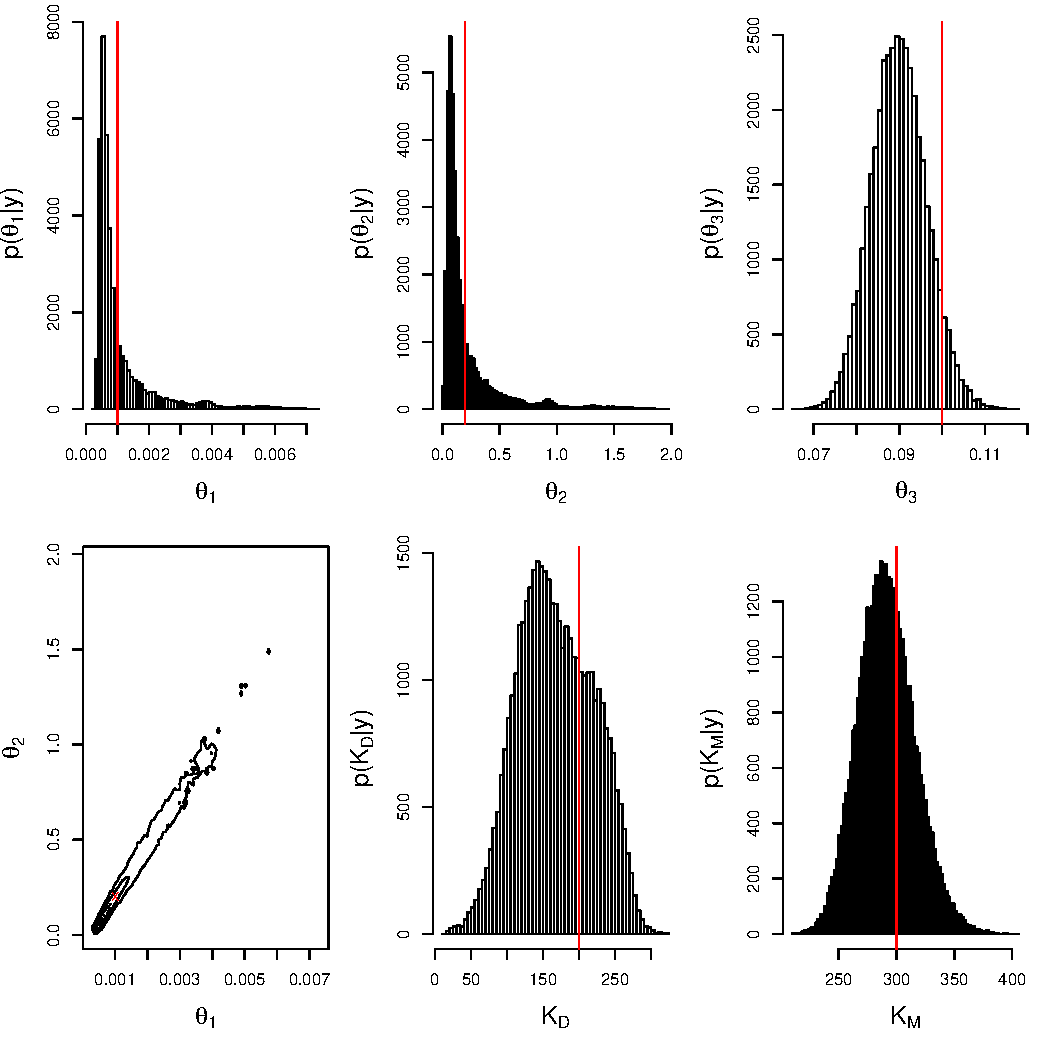
\includegraphics{Michaelis-Menton-parameter-posteriors} \pause
	\end{column}
	\begin{column}{0.5\textwidth}
	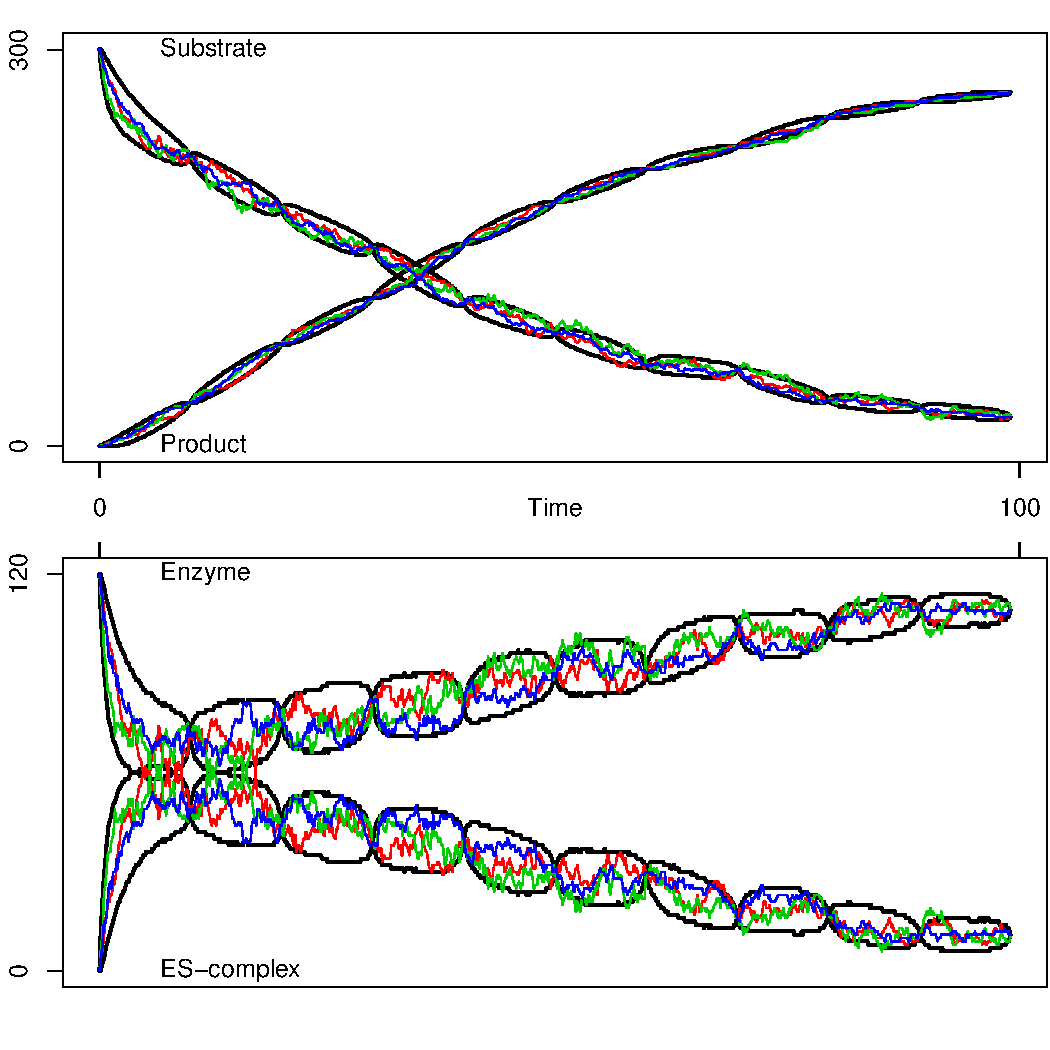
\includegraphics{Michaelis-Menton-trajectory-posteriors}
	\end{column}
	\end{columns}
}

\frame{\frametitle{}
	\setkeys{Gin}{width=0.8\textwidth}
	Since rejection sampling is inherently parallel, run this algorithm on a graphical processing unit: \pause 
	
	\vspace{0.2in}
	
	\begin{center}
	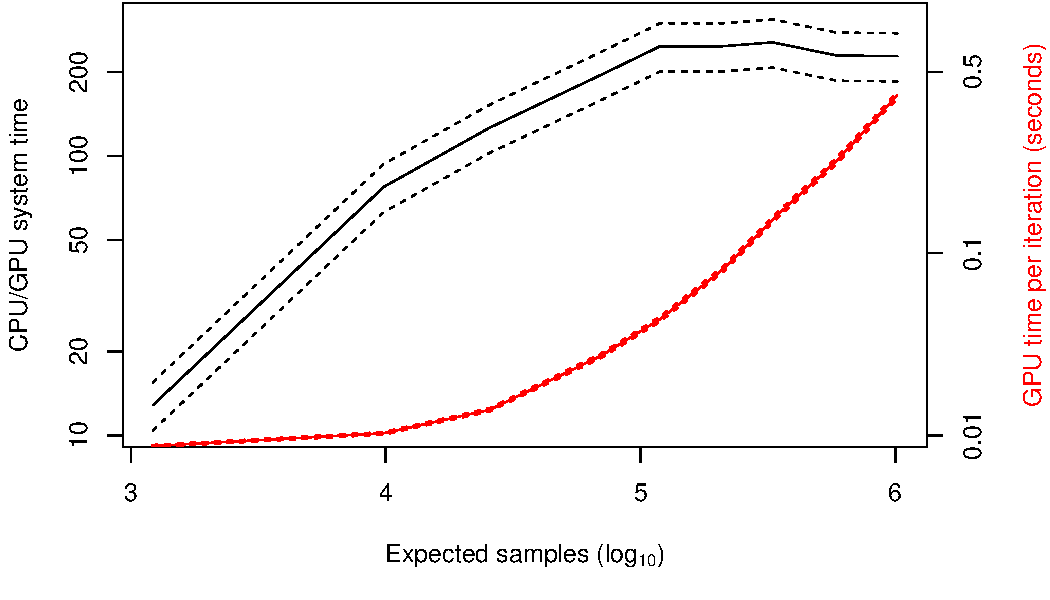
\includegraphics{Michaelis-Menton-CPUvsGPU}
	\end{center}
}

\section{Summary}
\frame{\frametitle{Summary}
	\begin{itemize}[<+->]
	\item Bayesian inference in discretely observed SCKMs
		\begin{itemize}
		\item Goal: $p(\theta|y)\propto p(y|\theta)p(\theta)$
		\item Likelihood, $L(\theta)=p(y|\theta)$, is analytically intractable 
		\item Sampling methods are required, e.g. rejection and/or Gibbs 
		\item Acceptance rate can be unacceptably low
		\end{itemize}
	\item Approximate Bayesian computation (ABC) in SCKMs
		\begin{itemize}
		\item Goal: $p(\theta|\rho\le\epsilon)\propto p(\rho\le\epsilon|\theta)p(\theta)$
		\item $\rho=\rho(y,X)$ measures the difference between data and a simulation
		\item $\epsilon$ balances computability with accuracy
		\item Readily accommodates bounded errors, e.g. $y_t=X_t\pm \epsilon$
		\end{itemize}
	\item ABC generally
		\begin{itemize}
		\item More general than SCKMs, e.g. phylogenetic trees
		\item Building $\rho$ is art, often use sufficient statistics of the data
		\item Not useful for unbounded errors, e.g. $y_t=X_t+\epsilon_t, \epsilon_t\sim N(0,\sigma^2)$
		\item Current debate about usefulness for model selection
		\end{itemize}
	\end{itemize}
}

\frame{\frametitle{}
\begin{center}
{\Huge Thank You!}
\end{center}

\vspace{0.2in}

Resources
\begin{itemize}
\item Niemi, Jarad and Wheeler, Matt. Efficient Bayesian inference in stochastic chemical kinetic models using graphical processing units. \url{http://arxiv.org/abs/1101.4242}
\item This presentation on BlackBoard Learn.
\end{itemize}
}

\end{document}


